%\begin{savequote}[8cm]
%Alles Gescheite ist schon gedacht worden.\\
%Man muss nur versuchen, es noch einmal zu denken.

%All intelligent thoughts have already been thought;\\
%what is necessary is only to try to think them again.
 % \qauthor{--- Johann Wolfgang von Goethe \cite{von_goethe_wilhelm_1829}}
%\end{savequote}

\chapter{\label{ch-theory}Theory}

\minitoc

%\section{Introduction}
\section{Introduction}
This section will briefly outline the key theory relevant to the later chapters of this thesis. It will start with an overview of the basic parameters governing laser physics, and of the interactions between plasmas and high powered lasers. There will then be a discussion of inertial confinement fusion, giving a basic overview of an ICF implosion and an introduction to some of the key concepts and ideas that will be explored in later chapters. This next section will discuss some of the most significant instabilities that affect such reactions.

The following section will then focus on how plasmas generally can be described mathematically. The kinetic description of plasmas will be introduced, before the fluid approximation (which is used in hydrocodes such as HYADES to model ICF implosions) is introduced. A brief description of the other key physics models used to describe plasmas in these simulations is also provided. Finally, the last section will discuss how shock waves occur in fluids, how these behave mathematically, and how they interact with material interfaces. This is key to the experiment described in the final section.

\section{Plasmas and laser-plasma interactions}
The basic definition of a plasma provided by Chen \cite{Chen2016} is `a quasi-neutral gas of charged and neutral particles that exhibit collective behaviour'. There are three major components to this definition. Firstly is that the plasma consists of charged and neutral particles, meaning that there is some degree of ionisation inherent to plasma material. This alone is not sufficient, and a plasma is distinct from an ionised gas. Quasi-neutrality means that the concentrations of charge or external plasmas are effectively `shielded' by the ions, such that the plasma can be considered neutral. Finally, the concept of `collective behaviour' means that plasma motions are not simply local, but can depend on conditions a long-way through the plasma (arising from the fact that the plasma consists of ions, whose motions will lead to electromagnetic forces that will propagate through the plasma). In this section some key concepts of plasma physics will be briefly introduced, which will illustrate these points further. The discussion here follows that in \cite{Chen2016}.

\subsection{The Debye length}
The Debye length $\lambda_D$ is a characteristic length scale in a plasma, defined by
\begin{equation} \lambda_D = \sqrt{ \frac{\epsilon_0 k_B T_e}{n e^2})}, \end{equation}
where $T_e$ is the electron temperature, $n$ is the number density of ions/electrons, $\epsilon_0$ is the permittivity of free space, and $k_B$ is Boltzmann's constant. The Debye length defines the (exponential-decay) length-scale over which charges are `shielded' by electrons within the plasma. Given that it is this electron shielding of charges which is responsible for quasi-neutrality, an approximate mathematical condition for a plasma can be written as 
\begin{equation} N_D = n \cdot \frac{4}{3} \pi \lambda_D^3 \gg 1, \end{equation}
where $N_D$ is the number of particles in a `Debye sphere', i.e. the number of electrons that would be in the Debye length of a charge, and thus available to shield it. Clearly for the charge to be effectively shielded and thus quasi-neutrality to be established, this number should be much larger than one.

\subsection{Plasma oscillations}
If the electrons in the plasma are displaced slightly from the stationary ions\footnote{Given the mismatch between the ion and electron mass in a typical plasma, when considering short time scales the ions are often considered to be stationary compared to the highly mobile electrons}, there will be a restoring force generated. This will accelerate the electrons towards the ions, which they will then overshoot - establish oscillations. The behaviour of such a wave can be calculated using the electron equations of motion\footnote{The electron equation of motion using the convective derivative, which is described later} and continuity and Poisson's equation,
\begin{equation} m n_e [\frac{\partial\vec{v_e}}{\partial t} + (\vec{v_e} \cdot \grad)\vec{v_e}] = -e n_e \vec{E} \end{equation}
\begin{equation} \frac{\partial n_e}{\partial t} + \grad \cdot (n_e \vec{v_e}) = 0 \label{eqn: ElectronEoM} \end{equation}
\begin{equation} \epsilon_0 \grad \cdot \vec{E} = e(n_i - n_e). \end{equation}
This set of equations is solved through linearisation, and results in sinusoidal oscillations of the electrons at the plasma frequency, 
\begin{equation} \omega_p \left( \frac{n_0 e^2}{\epsilon_0 m}\right). \label{eqn: PlasmaFrequency} \end{equation}

If a pressure term is added to the electron equation of motion (equation \ref{eqn: ElectronEoM}),
\begin{equation} \div P_e = 3 k_B T_e \div n_e, \end{equation}
then thermal motion of the electrons will cause the plasma oscillation to propogate as a plasma wave, with a dispersion relation described by
\begin{equation} \omega^2 = \omega_p^2 + \frac{3}{2} k^2 v_{th}^2, \end{equation}
where $k$ is the wave vector and $v_{th} = \frac{2 k_B T_e}{m}$. Such waves are known as plasma waves, electron waves, Langmuir waves, or plasmons. The existence of such waves serves to illustrate the collective behaviour that defines plasmas. Another condition for plasmas can be defined through $\omega_p \tau \gg 1$, where $\tau$ is the collision time between charged and neutral ions - such a condition essentially expresses that plasma oscillations must occur faster than collisions with neutral atoms, such that electromagnetic forces govern the motion rather than normal hydrodynamic forces.

A similar analysis can be used to derive a large range of possible oscillations in plasmas, in response to applied fields and electromagnetic waves\footnote{It should also be noted that while plasmas effectively shield electric fields, magnetic fields are undamped. External magnetic fields therefore lead to large number of potential plasma modes}. Two more particularly significant results are highlighted. First, if the derivation is performed for ions (rather than electrons), the ion-acoustic wave is obtained. This is equivalent to a sound wave in a plasma, and has the dispersion relation
\begin{equation} \omega = k v_s, \end{equation} where $v_s$ is the plasma sound speed. Secondly, the dispersion relation for an electromagnetic wave in a plasma is given by 
\begin{equation} \omega^2 = \omega_p^2 + c^2k^2. \end{equation}

It is significant that the dispersion equation for EM waves in a plasma contains the plasma frequency $\omega_p$. This means that only EM waves with a frequency higher than the plasma frequency can propagate into a plasma. As (according to equation \ref{eqn: PlasmaFrequency}) $\omega_p \propto \sqrt{n}$, this means that an an EM wave travels through plasma of increasing density, it will eventually encounter a `critical density' above which it cannot propagate in (i.e. the density for which the frequency of the incoming wave is equal to the plasma frequency). 

\section{Mathematical formulations of plasmas}

\subsection{The plasma distribution function}
Plasmas can be described in a number of different ways, each of which has their limitations. Here we will consider the full kinetic description of plasmas, and then highlight how the fluid approximation (which is used in radiation hydrodynamics codes to simulate plasmas over the timescales necessary for ICF) is obtained from this.

Variables such as the density of a plasma vary with it's position $\vec{r}$ (describing the three spatial dimensions $x,y,z$) and the time t. However, to fully describe the plasma, it's velocity distribution must also be considered. This is described by the `velocity distribution function' (or just the `distribution function') 
\begin{equation} f = f(\vec{r}, \vec{v}, t), \end{equation} 
where $\vec{v}$ is the velocity (consisting of the three dimensions consisting of $v_x, v_y, v_z$). $f$ can be used to find the number of particles per unit volume at position $\vec{r}$ and time $t$ with velocity components in a small range of velocities between $\vec{v}$ and $\vec{v} + d\vec{v}$ ($v_x$ and $v_x + dv_x$, $v_y$ and $v_y + dv_y$, $v_z$ and $v_z + dv_z$) through $f(\vec{r}, \vec{v}, t) d\vec{v}$.

The density $n$ of the plasma can thus be obtained by integrating $f$ over the entire velocity distribution,
\begin{equation} n(\vec{r}, t) = \int^{\infty}_{-\infty} f(\vec{r}, \vec{v}, t) d\vec{v}  = \int^{\infty}_{-\infty} \int^{\infty}_{-\infty} \int^{\infty}_{-\infty} f(\vec{r}, \vec{v}, t) dv_x dv_y dv_z. \end{equation}
In fact, a normalised version of $f$ is typically used - $\hat{f}$ - such that $\int^{\infty}_{-\infty} \hat{f}(\vec{r}, \vec{v}, t) d\vec{v} = 1$. This makes $\hat{f}$ a probability, and means that 
\begin{equation} f(\vec{r}, \vec{v}, t) = n(\vec{r}, t)\hat{f}(\vec{r}, \vec{v}, t). \end{equation}

\subsection{The Boltzmann and Vlasov equations}

Consider the evolution of the plasma distribution function $f$ with time. First, consider the collisionless. Taking the derivative $\frac{df}{dt}$ and rewriting the variables, the collisionless Boltzmann equation is obtained,
\begin{equation} \frac{\partial f}{\partial t} + \vec{v}\cdot \grad_x f + \frac{\vec{F}}{m} \cdot \grad_v f = 0. \end{equation}
Here, the acceleration term $\frac{d\vec{v}}{dt}$ has been expressed in terms of applied net force $F$ and mass $m$, in accordance with Newton's law. Collisions can be included by adding a term on the RHS, describing the rate of change of $f$ with time due to these collisions: 
\begin{equation} \frac{\partial f}{\partial t} + \vec{v}\cdot \grad_x f + \frac{\vec{F}}{m} \cdot \grad_v f = \left(\frac{\partial f}{\partial t}\right)_c. \end{equation}

Two special cases of the Boltzmann equation are particularly useful. Firstly, consider the case where collisions can be neglected (such as in a hot plasma), and where the only forces are electromagnetic. Then, the Boltzmann equation becomes
\begin{equation} \frac{\partial f}{\partial t} + \vec{v}\cdot \grad_x f + \frac{q}{m}(\vec{E} + \vec{v}\times\vec{B}) \cdot \grad_v f = 0, \end{equation}
which is known as the Vlasov equation. This equation can then also be further extended to include collisions with the addition of different collision operators $\left(\frac{\partial f}{\partial t}\right)_c$ - for instance the Fokker-Planck operator, which describes collisions from binary Coulomb collisions and thus forms the `Vlasov-Fokker-Planck equation'.

The Vlasov equation (with or without collision operators) can be simulated in so-called Vlasov codes, which calculate the velocity distribution of the plasma at each timestep. Such codes are useful for simulating kinetic effects in plasmas, such as Landau damping, which are not well described by other (more approximate) codes. However, such codes are computationally expensive, and it is not feasible to simulate them over the time and length scales necessary for an ICF implosion.

\subsection{The fluid equations}

%The fluid approximation makes the assumption that the velocity distribution of the plasma is assumed to be Maxwellian at all positions, and thus $\hat{f}$ can be described 
%\begin{equation} \hat{f} = (m / 2\pi KT)^{3/2} \exp{-v^2/v_{th}^2}, \end{equation} where $v = \sqrt{v_x^2 + v_y^2 + v_z^2}$ and $v_{th} = \sqrt{2KT/m}$.

The Boltzmann equation describes the evolution of the distribution function, which is the complete mathematical description of the plasma. Fluid variables, which vary as a function of $\vec{r}$ and $t$, can be obtained by taking moments of velocity of the distribution function (i.e. performing the integral $ \int^{\infty}_{-\infty} v^i f d\vec{v} $, where $i$ represents the moment being taken). The first three moments return the particle density $n$, fluid velocity $\vec{u}$, and pressure tensor $\vec{P}$:

\begin{equation} n = \int^{\infty}_{-\infty} f d\vec{v}  \end{equation}
\begin{equation} p = mn\vec{u} = \int^{\infty}_{-\infty} \vec{v} f d\vec{v} \end{equation}
\begin{equation} \underline{\underline{P}} = mn\vec{u} = \int^{\infty}_{-\infty} (\vec{v} - \vec{u})(\vec{v} - \vec{u}) f d\vec{v}.  \end{equation}

Fluid equations governing the evolution of each of these variables can also be obtained, by taking the equivalent moment of the Boltzmann equation. Under the fluid approximation, these equations are solved to describe the evolution of the plasma as a fluid; no knowledge of the distribution function is required.

The zeroth moment of the Vlasov equation is obtained by integrating each term (technically, this also requires multiplying by $v^0 = 1$). Doing this integration returns the \textit{continuity equation},
\begin{equation} \frac{\partial n}{\partial t} + \div (n \vec{u}) = 0. \end{equation}

Next, the Vlasov equation is multiplied by the first order moment, $m\vec{u}$. This results in the \textit{equation of motion,}
\begin{equation} mn(\frac{\partial \vec{u}}{\partial t} + (\vec{u} \cdot \grad)\vec{u}) = qn(\vec{E} + \vec{u} \times \vec{B}) - \div \underline{\underline{P}} + \underline{\underline{P}}_{ij} .\end{equation}

Finally, multiplying by the second order moment, $mv^2 / 2$, returns the energy equation,
\begin{equation} \frac{ \partial}{\partial t} (\rho \epsilon) = \div (\rho \vec{u} \epsilon) - \div (P \vec{u}) + \phi - \div \vec{F} + Q. \end{equation}
There are multiple ways to present this equation; the one presented here has had the kinetic energy subtracted from both sides, and has grouped terms into a dissipation function $\phi$ (containing material viscosities), and $Q$ is the energy exchange from collisions. The term $F$ is the heat flux, and $\epsilon$ is the internal energy of the fluid.

The fluid equations can be used to describe the evolution of the fluid variable directly, without consideration of the distribution function. However, note that the i'th order fluid equation always contains the (i+1)'th moment; the first-order equation of motion contains the second order Pressure term, while the second order energy equation contains the third order heat flux. Such a system of equations will therefore never form a closed set, and an additional equation is required to close it.

\section{Magnetohydrodynamics}
The equations in the previous section are sometimes referred to as the `two-fluid' equations, since there is a continuity equation and equation of motion for each of the two species (ions and electrons). A common approximation, Magnetohydrodynamics, can be obtained by making a series of assumptions. The basic outline of Magnetohydrodynamics is shown here, considering (for simplicity) a collisionless plasma and the first two moments of the Vlasov equation (this can be extended to include both collision operators, and the energy equation).

For Magnetohydrynamics, the continuity and equations of motion for the electron and ion fluids (with mass $m_s$, number density $n_s$ and charge $q_s$, where the species $s = i,e$ represents ions or electrons respectively) are combined into a single fluid. This fluid is described by it's mass density $\rho$, charge density $\sigma$, mass-averaged velocity $\vec{U}$, current density $\vec{J}$, and total pressure $\underline{\underline{P}}$. These four variables are calculated from the two ion species as
\begin{equation} \rho = m_i + m_e,  \end{equation}
\begin{equation} \vec{U} = \frac{m_i n_i \vec{u_i} + m_e n_e \vec{u_e}}{ m_i + m_e},  \end{equation}
\begin{equation} \underline{\underline{P}} = \underline{\underline{P}}^i + \underline{\underline{P}}^e,  \end{equation}
\begin{equation} \sigma = q_i n_i + q_e n_e,  \end{equation}
\begin{equation} \vec{J} = q_i n_i \vec{u_i} + q_e n_e \vec{u_e}.  \end{equation}

Continuity equations for the single-fluid can be obtained by summing the individual continuity equations for the ions and electrons. This gives the \textit{conservation of mass} equation,
\begin{equation} \frac{\partial \rho}{\partial t} + \div (\rho \vec{U}) = 0. \end{equation}
A conservation of momentum equation can likewise be obtained, by summing the equations of motion for the two individual species,
\begin{equation} \frac{\rho \vec{U}}{\partial t} + (\vec{U} \cdot \grad)\vec{U} =\vec{J} \times \vec{B} - \div \underline{\underline{P}} .\end{equation}

An equation for the current density is obtained by multiplying the ion and electron equations of motion by the relevant charge over mass $q_s/m_s$, and summing the two. The algebra for this is complicated, and to reach the final equation some of the key assumptions of ideal MHD are required:
\begin{itemize}
	\item{The plasma is quasi-neutral, such that $\sigma$ is approximately zero (this has the effect that Gauss' law, $\div \vec{E} = \sigma / \epsilon_0$, cannot be used over large length scales in the plasma).}
	\item{The length scales and time scales of interest in the plasma are large (i.e. much longer than the period of a plasma oscillation, or a debye length).}
	\item{The effects of electron inertia are negligible, i.e. $m_e \ll m_i$.}
\end{itemize}
Applying these assumptions and completing the algebra allows the \textit{Generalised Ohm's law} to be derived, 
\begin{equation} \vec{E} = -\vec{U}\times\vec{B} + \frac{\vec{J} \times \vec{B}}{n_e} - \frac{\div \underline{\underline{P}}^e}{n_e}. \end{equation}










\section{Additional physics models required for hydrocodes}

The previous sections describe how plasmas can be modelled mathematically, and how the fluid approximation can be used to enable simulations of an ICF implosion. This thesis will discuss a number of simulations using HYADES, a radiation-hydrodynamics code that operates on this principle. However, the equations in the previous sections are not sufficient for a complete description of all the processes involved in a plasma, and further physics models are required to conducts a simulation. This chapter will briefly summarise some of the other important physics required to describe a plasma (based on the more complete descriptions provided in \cite{Colvin2013}), while also highlighting the particular models used in the HYADES simulations presented in this thesis.

\subsubsection{Discretisation of the plasma}
The above description treats the relevant variables as continuous parameters, but to simulate the plasma it is necessary to discretise the plasma and it's relevant variables. There are two formalisms which can be used; Eulerian and Lagrangian. In an Eulerian formalism, the change in variables at a particular point is measured; the change in a variable as the plasma flows through this point (even if the plasma itself is not undergoing change) must therefore be considered. A Eulerian fluid code therefore consists of a fixed mesh, and the plasma flows through it. In the Lagrangian formalism, we instead track changes at specific points in the plasma. If the plasma moves, the mesh follows it; and thus the mesh moves with the plasma and the mass of each zone remains constant. Hyades is a Lagrnagina fluid code.

\subsubsection{Laser propagation and absorption}
Hydrocodes typically use a ray tracing model to describe incoming laser beams, and track the laser absorption. The critical density of associated with the laser frequency places a limit on how far into a plasma the light can propagate before it is reflected\footnote{While the laser initially is incident on a solid surface, the laser will quickly ablate away some solid material. This establishes a `coronal plasma', with a density gradient that increases towards the main fuel. The incoming laser now travels through this plasma, and the laser absorption processes occur within this plasma.}.

The coronal plasma is partially or fully ionised, meaning that there are both bound and free electrons that the incoming light can interact with. At the lower end of `high intensity' (high intensity defined here as around $10^{13}$ \unit{\watt\per\centi\meter\squared} and above), the photon energy is low compared to the ionisation potential and so absorption by free electrons dominate. Inverse Brem{\ss}trahlung is thus the most significant absorption mechanism; this is a collisional process, where a free electron is accelerated by a photon, in a process mediated by a nearby ion (the reverse of the more famous Brem{\ss}trahlung radiation). Inverse Brem{\ss}trahlung scales as $T_e^{-3/2}$, and thus absorption through this process decreases as the temperature increases. This is the mechanism through which most energy is absorbed in ICF applications.

Other absorbtion processes also play a role. Resonant absorption occurs very close to the critical density surface, where the plasma frequency matches the frequency of the laser, and thus Langmuir waves can be excited\footnote{Say something about the cos dependence}. This is a collisionless process, and becomes more significant at higher temperatures. Other mechanisms also become significant at high intensity, and see the incoming EM wave excite a range of plasma modes; these are termed `parametric instabilities', and will be treated in a later section.

\subsubsection{Radiation transport}
Radiation hydrodynamics codes treat the radiation as a third fluid, which can exchange energy and momentum with the ion and electron fluids. The key parameter to describe the radiation is the specific intensity, $I(\vec{r}, \upsilon, \vec{\Omega}, t)$ where $\upsilon$ is the frequency and $\Omega$ are two angular coordinates. This quantity is an energy flux, and it can thus be expressed as a distribution function through 
\begin{equation} I_{\upsilon}(\vec{r}, \vec{\Omega}, t) d\upsilon d\vec{\Omega} = h \upsilon c f(\vec{r}, \upsilon, \vec{\Omega}, t), \end{equation}
where $I_{\upsilon}$ is the spectral intensity for a given frequency.

This third fluid is coupled to the other fluids by adding a radiation flux term $F_{\upsilon}$ to their energy conservation equations. The inclusion of an extra variable means that an additional equation must be included in order to close the set. This new equation is the radiation transport equation - the equation of motion for the photons in the radiation fluid. This equation is expressed as 
\begin{equation} \frac{1}{c} \left( \frac{\partial I_\upsilon}{\partial t} + c \vec{\Omega} \cdot \grad I_{\upsilon} \right) = \rho \kappa_\upsilon' [B_\upsilon (T) - I_\upsilon], \end{equation} where $B_\upsilon (T)$ is the black-body intensity at frequency $\upsilon$ for a temperature T, and $\kappa_\upsilon' = \kappa_\upsilon ( 1 - \exp{-h\upsilon / k_B T})$ where $\kappa_\upsilon$ is the absorption coefficient.

This equation cannot be solved exactly, and so approximations are required. The most common is the diffusion approximation, which assumes that the total radiation flux is isotropic and thus the net flux is zero. This assumption is valid for optically thick plasmas, and allows the radiation transport equation to be converted into the diffusion approximation, which can be solved by a simulation code (this derivation is not reproduced here). 

However, to solve the diffusion equation the emission, absorption and scattering coefficients must be calculated. These variables are each continuous in frequency - this is resolved in the derivation by averaging the quantity over a frequency range\footnote{The `Planck mean' is used for optically thin plasmas, while the `Rosseland mean` is used when the plasma is optically thick.}. These variables can vary by many orders of magnitudes as a function of frequency, and thus a single average is often a poor approximation. As such, radiation hydrodynamics codes such as HYADES use `multi-group' radiation transport, where a number of frequency groups are specified, and a separate average absorption coefficient is calculated for each group.

\subsubsection{Thermal transport}

The second moment of the Boltzmann equation gives the energy transport equation. In 1D, and subtracting the kinetic energy, this has the form
\begin{equation} \frac{ \partial}{\partial t} (\rho \epsilon) = \div (\rho \vec{u} \epsilon) - \div (P \vec{u}) + \phi - \div \vec{F} + Q, \end{equation}
where $\phi$ is a dissipative term arising from viscosity, and Q is the energy exchange between particles from collisions. $\vec{F}$ is the heat flux, which can be described using Fourier's law 
\begin{equation} \vec{F} = - \chi \grad T, \end{equation} where $\chi$ is the thermal conductivity constant. To solve this equation, the thermal conductivity must be known.

The most commonly used thermal transport model is the Spitzer-H{\"a}rm model, which assumes that the Fokker-Planck equation can be used to find the collision term and that the velocity distribution is a Maxwellian with a small perturbation, allowing the transport coefficients to be calculated. This model finds that $\chi \propto \frac{T^{5/2}}{\ln{\Lambda}},$ where the denominator is the `Coulomb logarithm'.

However, the Spitzer-H{\"a}rm model overestimates electron heat transport into cold-dense material in the  presence of large temperature gradients. This can result in electron fluxes above the `free streaming limit'  - the maximum possible flow of thermal energy. To account for this, hydrodynamic simulations typically apply a flux-limiter; a parameter set with a value typically around 0.05. The simulation code will then use the smaller value of either the Spitzer-H{\"a}rm solution, or the free-streaming flux multiplied by this flux-limiter.

\subsubsection{Ionisation}
As the laser passes through the coronal plasma, it will also serve to ionise material. There are a variety of mechanisms through which this can be performed. Generally the photon energies are not high enough to liberate electrons directly, and thus multi-photon ionisation processes are required. As the electric field associated with the laser becomes comparable to the Coulomb barrier trapping the electron. This barrier can become sufficiently perturbed by the field E that at some distance from the electron position, the barrier is lower than the electron energy; in this case, the electron can quantum-mechanically tunnel through the barrier, and escape in a process known as tunnel ionisation.

Modelling the ionisation state of the plasma can also be performed through a range of models. The Saha equation can be used to estimate the relative populations of ionisation levels for low-density plasmas at high temperatures in local thermal equilibrium; however, it struggles away from these criteria. The Thomas-Fermi ionisation model considers an electron gas consisting of free and bound electrons, and treats this gas as using Fermi-Dirac statistics (as opposed to the Boltzmann statistics used by the Saha equation). The model used for the simulations in this thesis is an average atom LTE ionisation model. This model, rather than attempt to find the shell populations of many different atomic configuration, considers a single average-atom with a few discrete energy levels. The average-atom is not real; it can have a non-integer number of bound electrons in each level, in order to best approximate the average over all the atomic configurations. It includes a model for electron screening and LTE (local thermodynamic equilibrium) equations are used to calculate the average shell populations. 

\subsubsection{Equation of state}
The equation of state needs to be evaluated for the equations to be closed; this means being able to determine the material pressure as a function of it's density and temperature. This is done through determining the partition function describing a material, using thermodynamic relations to determine the free energy, and then using this to calculate the pressure, internal energy and entropy as a function of the density and temperature.

There are a number of potential EOS models. A simple common model is the Thomas-Fermi equation of state; this assumes all electrons (free and bound) can be treated as a single fluid obeying Fermi-Dirac statistics, and all the ions are treated as nuclei obeying Boltzmann statistics. This model is simple to evaluate, and is a reasonable description for high ionisation and high temperature plasmas. One of the key limitations is that it does not include coupling forces, and thus it is a poor description of low-temperature solids. Another important EOS model is the Gr{\"u}neisen equation of state, which treats solids where the atoms are held in a lattice structure. This formulation treats the pressure and energy in the solid as a sum of compressional and thermal components, and defines a Gr{\"u}neisen parameter $\Gamma$ which is used to define the material and is proportional to the ratio of it's thermal pressure to it's thermal energy. The Gr{\"u}neisen EOS can be used to describe low-temperature solids, but it assumes that the movement of the atoms around the equilibrium positions are small and thus breaks down as the thermal motion of the atoms increases.

It is clear that the equation of state is a complicated topic. More complicated models exist based on the quotidian Equation of State (QEOS). This uses a modified Thomas-Fermi model with a bonding correction term to describe the electrons, while combining a number of models (including the Gr{\"u}neisen EOS) to describe the ions - producing an EOS that is multi-phase and thermodynamically consistent. Many variations of this model exist. 

Hydrocodes such as Hyades provide a number of options for the equation of state, but there are two main ones for ICF work. Firstly, many codes accept tabulated equation of state data - such as SESAME tables, which are maintained for a number of materials by Lawrence Livermore National Laboratory. These use complicated first-principle (and often QEOS) models, which are also compared to experiments. Alternatively, HYADES also provides an in-line QEOS model that can be used. Both approaches are used for different materials in this thesis.

\section{Basic description of inertial confinement fusion}

In inertial confinement fusion, a driver is used to compress a capsule containing deuterium-tritium fuel to high pressures, densities and temperatures. In direct-drive ICF, this driver is a laser which irradiates the plasma directly. In indirect-drive ICF, the laser is incident on the inside of a hohlraum, generating a bath of x-rays which then irradiate the capsule. In either case, the intense electromagnetic radiation ablates the outer surface of the plasma. This ablation and expansion of material accelerates the remaining material inwards, compressing the capsule \cite{Atzeni2008}. The driver is typically designed to provide a pressure vs time profile such that a serious of shocks are generated to compress the capsule at different times; the use of multiple shocks reduces the amount of entropy injected into the fuel, allowing high densities to be achieved than is possible with a single shock.

The capsule typically consists of a central DT-vapour region. This is then surrounded by a layer of cold dense DT fuel (ice in many cases, or liquid DT-wetted-foams as is the focus of this thesis), which in turn is typically surrounded by an ablator layer. The high density ablator is used to absorb the radiation and accelerate the rest of the material inwards effectively. This thesis will focus on `central hotspot ignition', where as the capsule implodes it forms a central `hotspot' (consisting of high temperature but low-temperature material) and a surrounding `shell' consisting of high density but low temperature material.

As the capsule implodes, the pressure in the center of the capsule will begin to increase. This will cause the shell to begin to decelerate, and the shell kinetic energy will be converted into thermal energy within the hotspot. Eventually the shell will come to a complete stop, at the time of maximum compression, before beginning to explode outwards. The fuel is `confined' for this brief period before inertia, before it rapidly begins to disassemble. 

If the temperature and density within the hotspot are sufficiently high, fusion reactions will begin to occur. When DT fuel is used as described here, the dominant reaction is \begin{equation} D + T \rightarrow \alpha(3.5 \text{MeV}) + n(14.1 \text{MeV}), \end{equation} where D is a deuterium ion, T is a tritium ion, $\alpha$ is an alpha particle (helium ion) and $n$ is a neutron \cite{Atzeni2008}. This reaction generates 17.6 MeV which is distributed between the kinetic energy of the neutron and the alpha particle. DT fuel is chosen because this reaction has the largest cross section at low energies.

The neutron has a low chance of absorption, and thus escapes from the fuel assembly. The alpha particle however can be reabsorbed by the plasma. This adds 20 \% of the 17.6 MeV generated from the fusion reaction back into the system, further heating it. Alpha heating thus provides the instability central to fusion, adding more energy so that further fusion can occur. A balance of energies in the hotspot shows that $\alpha$ particle `self-heating' overtakes the losses in the hotspot (due to Bremsstrahlung) at around 4.3 keV for a pure DT plasma\footnote{Bremsstrahlung emission scales with atomic number $Z$ as $Z^2$, and so the presence of heavier ions in the hotspot will lead to higher required temperatures.}. This instability is referred to colloquially as ignition. In central hotspot ignition, the hotspot undergoes this process, and then generated alpha particles heat the cold-dense shell, inspiring further fusion reactions and generating a propagating burn wave that travels out from the center of the capsule.

The plasma conditions required to achieve ignition were first quantified by Lawson \cite{Lawson1957}, who estimated the temperatures and densities based on the power balance in a reactor. This is most commonly expressed through the famous `triple product' 
\begin{equation} n \tau_E T \approx 3.3 \times 10^{15} \; \unit{\centi\meter\cubed} \; \unit{\second}\; \text{keV}, \end{equation}
for a temperature $8 < T < 25 $keV and where $n$ and $\tau_E$ are the density and plasma confinement time respectively. However this expression is more suited to magnetic confinement fusion. For ICF, ignition instead needs to focus on the hotspot conditions - the hotspot must be large enough for self-heating to occur, and to produce enough energy to launch the propagating burn wave. This requires a large number of the alpha particles to be absorbed within the hotspot, leading to conditions on the areal density $\rho R$ (the integral of density with radius over a specified volume, and proportional to how much fuel an alpha particle would need to pass through to escape) and temperature $T$ of the hotspot. A variety of measures of `margin' (or how well a capsule is performing) have been developed and used for ICF, but a simple and often quoted one is that presented by Cheng \textit{et al.}:
\begin{equation} \left( \rho R \right)_\mathrm{HS} \geq 4 \frac{\kappa_\mathrm{C}}{f_\mathrm{T}} \left( \frac{T}{\mathrm{keV}} \right)^{-2.5} \text{ \si[per-mode=symbol]{\gram\per\centi\meter\squared}}, \label{ChengEqn} \end{equation}
where $\kappa_\mathrm{C} \simeq 5.514$ is a constant depending on the power law approximation for DT reactivity, and $f_\mathrm{T} \propto \sqrt{ \rho_\mathrm{p} / \rho_\mathrm{HS}}$ is a tamping factor (typically assumed to be 1 for basic estimates of ignition threshold) \cite{Cheng2014}. This quantifies ignition in terms of the temperature $T$ and areal density $\rho R$ of the DT fuel within the hotspot. This formula suggests that for an ion temperature of $T_{hs} \approx 4 \text{keV}$, a hotspot density of approximately $(\rho R)_{hs} \approx 0.3 \unit{\gram\per\centi\meter\squared}$ is required.

The above equation quantifies whether ignition will occur based on the hotspot parameters only. To produce high gain ignition alone is not sufficient; the capsule shell must contain a large amount of compressed DT fuel, and a large quantity of this must be burnt up before the fuel disassembles. Ignition sparks the burn wave through this dense fuel, but how efficiently it burns depends upon the shell conditions. This can be quantified using the fuel burn-up fraction $\Phi$, which compares the number of fusion reactions that occur to the total number of DT ion pairs in the capsule (i.e. the maximum number of potential reactions). This is typically estimated as 
\begin{equation} \Phi = \frac{ \rho R} {6.3 + \rho R}, \end{equation}
where in this case $\rho R$ is the areal density of the full fuel assembly (i.e. hotspot and shell) \cite{Fraley1974}. Using this equation, it is evident that the shell areal density must be around 3~\si[per-mode=symbol]{\gram\per\centi\meter\squared} in order to achieve a burn up factor of around 0.3. This highlights that both the hotspot and shell conditions are important to achieving a high-gain igniting capsule.

\subsection{Alternative ignition schemes}
In central hotspot ignition, as described above, the driver fulfills the dual roles of fuel compression and hotspot formation simultaneously. This leads to stringent symmetry requirements. Alternative ignition designs have been proposed which separate these two processes; two key concepts are described below.

In fast ignition \cite{Tabak1994}, a laser driver is used to compress the fuel to high density. A lower laser power is used, and the fuel is compressed instead into an isochoric assembly at much lower velocity - giving a sphere of fuel of roughly constant density throughout. The low laser power and more moderate accelerations serve to prevent significant instability growth. A particle beam is then used to heat a small volume at the fuel surface to high temperature; this forms the hotspot, generates fusion reactions, and causes a burn-wave that propagates through the rest of the fuel \cite{Tabak2005, Tabak2006}. The particle beam could be formed of electrons or ions. Schemes have also been proposed using cones to allow the particle beam to irradiate fuel at the center of the assembly \cite{Kodama2002, Kitagawa2002}, rather than at the surface (so called `cone-in-shell' fast ignition). A major challenge to achieving fast ignition is generating and transporting the particle beams, and using them to heat the fuel efficiently \cite{Norreys2014}.

Another scheme that has generated significant interest is shock ignition \cite{Betti2007}. Here, lower laser powers are again used to compress the fuel at lower velocities, reducing hydrodynamic instability growth - but unlike fast ignition, the compression is isobaric (such as in central hotspot ignition). However, a late high intensity laser pulse is then applied to drive an extremely strong final shock through the fuel, resulting in high temperatures in the center of the capsule and generating the hotspot. This design is conceptually similar to central hotspot ignition, but allows the fuel to be assembled without such hydrodynamic instability concerns. The main concern for shock ignition is that the high intensity of the late laser pulse can results in significant parametric instabilities, which could lead to hot electron generation and preheating of the fuel. An alternative scheme - shock augmented ignition - has recently been proposed to mitigate this, where a dip in the laser power is used before the final shock \cite{Scott2022}. This dip means that the laser intensity can then be increased to more moderate levels while still generating the strong shock (it is the increase in intensity that is important, rather than the absolute value), and thus the high levels of parametric instability can be avoided.







\section{Instability growth}
The key challenge for achieving high-performing ICF implosions is the prevention, mitigation and control of instabilities. Instabilities are effects beyond the pure compression and burn physics discussed in the previous section, which typically result in reductions in fusion performance beyond what would otherwise be expected. Instability growth a the key reason that the National Ignition Campaign did not perform as intended \cite{Lindl2014, Hurricane2014}.

There are two major classes of instability growth which affect ICF implosions. Hydrodynamic instabilities are the unstable growth of perturbations in the flow of the plasma as the capsule implodes, and are discussed in Section \ref{Hydro instabilities}. Parametric instabilities arise from non-linear interactions between the incoming laser and the plasma, and will be discussed in Section \ref{Parametric instabilities}

\subsection{Hydrodynamic instabilities} \label{Hydro instabilities}
As the ICF capsule is compressed and implodes, small perturbations arise which can grow unstably and significantly affect the course of the implosion. These hydrodynamic instabilities can cause a number of potential degradation mechanisms. They can cause significant asymmetry of the implosion, leading to non-uniform (and reduced) compression, and can in extreme cases lead to the break-up of different layers of material within the capsule. They can also lead to the mixing of the different layers (such as of ablator material into the cold DT fuel layer, or of cold fuel into the hotspot). These effects can significantly degrade fusion performance \cite{Ma2013}.

The most significant hydrodynamic instability for ICF is the Rayleigh-Taylor instability, which occurs when a fluid of low density is accelerated into a fluid of high density. Small perturbations will undergo rapid growth, leading to `spikes' at the interface of the two materials \cite{Atzeni2008}. This leads to mixing of the layers, and in extreme cases can lead to the complete break-up of the layers. RT instability occurs both at the outer edge of the shell throughout the implosion, and at the shell/hotspot boundary late in the implosion. Fortunately RT growth at the capsule outer surface is reduced due to ablative-stabilisation where the ablation of the surface reduces the perturbations as they grow, although this is not sufficient to prevent RT growth completely. The ablation-stabilized growth rate for the RT instability can be expressed as
\begin{equation} \gamma = \alpha \sqrt{ak} - \beta k u_\mathrm{a}, \label{eq:RTI} \end{equation}
where $a$ is acceleration, $k$ is the wave number of the perturbation, $\alpha$ and $\beta$ are numerically determined coefficients, and $u_\mathrm{a}$ is the ablation velocity \cite{Takabe1985, Betti1998}.

RT instability growth is `seeded' by small initial perturbations, which can arise from a number of possible factors \cite{Haines2019a}. These include asymmetries in the laser (or x-ray) drive, small perturbations to the capsule (such as pits/voids), the capsule fill-tube (a small tube used to fill the capsule with the DT fuel), and the capsule support tent (i.e. the material used to hold the capsule in place). Efforts are made to minimise and control all possible RT seeds as much as possible to prevent and minimise instability growth.

Other hydrodynamic instabilities also affect ICF capsules, albeit to a lesser extent \cite{Atzeni2008}. The Richtmeyer-Meshkov instability occurs when a shock wave crosses between two materials and the interface is not-perfectly flat; the velocity of the surface is thus non-uniform, and the perturbations grow. These perturbations can then in-turn seed RT instability growth. Another example is the Kelvin-Helmholtz instability, which occurs when there is show flow between two different fluids. This can occur as RT `spikes' propogate and grow, and can thus play a role in the development of the later stages of this growth.

\subsection{Parametric instabilities} \label{Parametric instabilities}
Parametric instabilities instead arise from laser-plasma interactions. When high-intensity light passes through the ablated/coronal plasma, plasma modes (such as those described in \hl{Section} can be excited. This can result in reduced absorption of laser light, less symmetry in the drive (which can thus lead to less uniform compression, and seed hydrodynamic instabilities), and preheating of the fuel (again reducing performance). The incoming EM wave can excite a number of modes (including scattered EM waves), according to the wave vector and frequency matching conditions:
\begin{equation} k_0 = k_2 \pm k_1, \end{equation}
\begin{equation} \omega_0 = \omega_2 \pm \omega_1. \label{eqn: freq matching} \end{equation}
$k$ is the wave vector and $\omega$ is the angular frequency, while the subscript 0 represents the initial wave and 1 and 2 repesent the excited modes \cite{Chen2016}. The discussion in this section follows that in \cite{Chen2016} and \cite{Craxton2015}.

\subsubsection{Stimulated Raman scattering (SRS)}
In stimulated Raman scattering, the incoming electromagnetic wave scatters from a Langmuir wave (or plasmon), producing a scattered photon. By substituting into Equation \ref{eqn: freq matching} the dispersion relations for the EM waves ($\omega_0 = \omega_p + c^2 k_0^2$ for the incident wave, and $\omega_2 = \omega_p + c^2 k_2^2$ for the scattered wave) and the Langmuir wave ($\omega_1 = \omega_p + \frac{3}{2} v_{th}^2 k_e^2$) discussed in \hl{Section}, it is clear that $\omega_o < 2 \omega_p$. The SRS instability therefore only occurs for densities below the quarter critical density, $n < n_c / 4$. SRS  leads to Langmuir waves, which (after undergoing wave-breaking) can result in fast moving `hot' electrons \cite{Rosenberg2018}. These electrons can travel significant distances before being absorbed and can therefore result in preheating of the cold DT fuel within the capsule, which makes it harder to compress and reduces fusion performance.

\subsubsection{Two-plasmon decay (TPD)}
In two-plasmon decay, where the instability is generated by the scattering of two plasmons (with no scattered EM wave). This requires that $\omega_0 \approx 2\omega_p$, which means that the instability is only possible over a small density range around the  quarter critical density. As with SRS, this instability can lead to preheating of the cold DT fuel through the generation of hot electrons \cite{Yaakobi2000}.

\subsubsection{Stimulated Brillouin scattering (SBS)}
In stimulated Brillouin scattering, the incoming EM wave scatters into a ion-acoustic wave and a scattered EM wave. Since the frequency of an ion-acoustic wave is relatively small ($\omega_{IA} = kv_s$), the frequency of the scattered EM wave is only slightly lower than that of the incident wave, and the instability can occur throughout the entire coronal plasma. SBS is a significant instability for ICF due to it's role in cross-beam energy transfer (CBET), where it moderates the transfer of energy between different incoming laser beams - an effect which can reduce the absorption of laser light by 10-20\% \cite{Igumenshchev2012}.

\subsubsection{Mitigation of parametric instabilities}
Parametric instabilities are generated when high intensities of EM radiation pass through a plasma. There is thus a threshold above which these processes begin to occur in significant quantities, and they can be mitigated by keeping the intensity below this value. However, this can be challenging to balance with the high intensity demands of ICF. Alternatively, parametric instabilities can be mitigated by using high bandwidth lasers, so that the intensity is spread over a wider range of frequencies \cite{Follett2018}. This keeps the intensity of individual frequencies under the threshold, and is seen as a key instability-mitigation strategy for direct-drive in the future \cite{Campbell2021a}.


\section{Shocks and impedance matching}

\subsection{Shock physics}

Shocks, referring to a sudden change in plasma properties over a thin transition region, are ubiquitous in plasmas and inertial confinement fusion, occurring whenever there is a change in the pressure applied to the capsule. Generating and measuring the plasma state produced by a shock was also the key feature of the experiment described in \hl{SECTION}. As such, this section will provide a brief overview of the key principles of shock physics, based on the explanation in \cite{Zeldovich1966}.

\begin{figure}
\centering
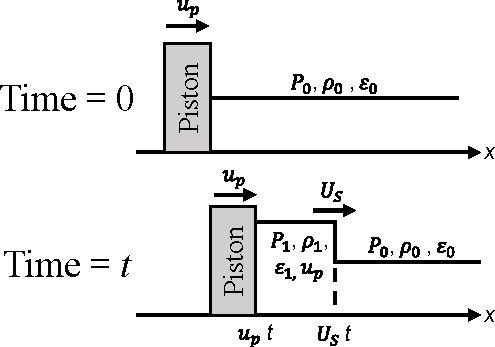
\includegraphics[width=0.6\textwidth]{figures/Theory/Piston.pdf}% Here is how to import EPS art
\caption{\label{fig:Piston} A piston, moving at velocity $u_p$ drives a shock through a medium. The shock moves at velocity $U_S$, leaving material behind it in a new shock state denoted by the subscript 1. Based on a diagram in \cite{Zeldovich1966}.}
\end{figure}

Consider the situation in Figure \ref{fig:Piston}. The material is initially at rest, until it is disturbed by a piston moving at velocity $u_p$, and applying a pressure $P$. After a time $t$, the piston has moved by a distance $ut$. This drives a disturbance (shock) through the material with a `shock velocity' $U_S$, which is now at the position $U_S t$. Behind the shock the material is at the piston pressure and velocity $P$ and $u_p$, and at a new higher density $\rho_1$. Ahead of the disturbance, the material is unaffected. As the newly shocked material moves at velocity $u_p$, this quantity is known as the `particle velocity'.

Three equations can be derived based on the conservation of mass, momentum, and energy across the disturbance. Considering that the mass in distance $U_S t$ cannot have changed, the expression
\begin{equation} \rho_0 U_S = \rho_1 (U_S - u_p) \end{equation}
is obtained. (Here, as in the following equations, $t$ and the area $A$ cancel from both sides of the equation. Considering the momentum of this material (which changes according to the impulse, arising from the difference in pressure either side of the boundary), leads to the equation 
\begin{equation} \rho_0 U_S u_p = P_1 - P_0. \end{equation}
Finally, considering the change in total energy (both internal energy $\epsilon$ and kinetic energy), which must equal the work applied by the piston as it moves the distance $ut$, results in the third equation 
\begin{equation} \rho_0 U_S (\epsilon_1 - \epsilon_0 + \frac{u_p^2}{2}) = P_1 u_p. \end{equation}

These equations relate the four shock variables $U_S$,$u_p$,$P$ and $\epsilon$ to one another. If the state of the material ahead of the shock is known, then finding any two of these variables allows the other to be calculated. They are referred to collectively as the Rankine-Hugoniot relations. They were derived here in a stationary frame (where the shock moves with velocity $U_S$), and are typically expressed as
\begin{equation} \rho_1 = \frac{\rho_0 U_S}{U_S - u_p}, \label{eqn: RH1 stationary} \end{equation}
\begin{equation} P_1 - P_0 = \rho_0 U_S u_p, \label{eqn: RH2 stationary} \end{equation}
\begin{equation} \epsilon_1 - \epsilon_0 = \frac{P_1 u_p}{\rho_0 U_S} - \frac{u^2}{2}. \label{eqn: RH3 stationary} \end{equation}

\subsection{Rankine-Hugoniot relations in a moving frame}

\begin{figure}
\centering
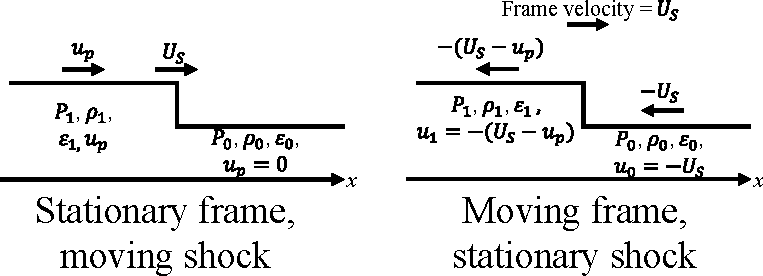
\includegraphics[width=0.8\textwidth]{figures/Theory/ReferenceFrames.pdf}% Here is how to import EPS art
\caption{\label{fig:ReferenceFrames} The shock as viewed in the two frames. In the stationary frame, the shock moves with velocity $U_S$, the shocked material with velocity $u_p$, and the unshocked material is stationary. In the moving frame, the shock is stationary, the shocked material has velocity $u_1$, and the unshocked material has velocity $u_0$. The other variables are unchanged.}
\end{figure}

Alternatively, the same equations can be considered in a moving frame, where the shock is stationary. The frame now moves at velocity $U_S$, as displayed in Figure \ref{fig:ReferenceFrames}. This means the unshocked material moves into the stationary shock front at a velocity $u_0 = -U_S$, while the material behind the shock moves away at the slower velocity $U_1 = -(U_S - u_p)$. This transformation can be applied to each of Equations \ref{eqn: RH1 stationary}, \ref{eqn: RH2 stationary} and \ref{eqn: RH3 stationary} to give the Rankine-Hugoniot relations in an alternative form,
\begin{equation} \rho_1 u_1 = \rho_0 u_0, \label{eqn: RH1 moving} \end{equation}
\begin{equation} P_1 + \rho_1 u_1^2 = P_0 + \rho_0 u_0^2, \label{eqn: RH2 moving} \end{equation}
\begin{equation} \epsilon_1 + \frac{P_1}{\rho_1} + \frac{u_1^2}{2} = \epsilon_0 + \frac{P_0}{\rho_0} + \frac{u_0^2}{2}. \label{eqn: RH3 moving} \end{equation}
These three relations can also be derived by integrating over the differential equations describing the conservation equations given in \hl{SECTION}.

These equations can be further manipulated to derive some other useful expressions. Equations \ref{eqn: RH1 moving} and \ref{eqn: RH2 moving} can be used to find new expressions for the velocities $u_1$ and $u_0$, 
\begin{equation} u_1^2 = \nu_1^2 \frac{P_1 - P_0}{\nu_0 - \nu_1}, \label{eqn: RH moving u1} \end{equation}
\begin{equation} u_0^2 = \nu_0^2 \frac{P_1 - P_0}{\nu_0 - \nu_1}, \label{eqn: RH moving u0} \end{equation}
where $\nu$ is the specific volume, $\nu = \frac{1}{\rho}$. Substituting Equations \ref{eqn: RH moving u1} and \ref{eqn: RH moving u0} into Equation \ref{eqn: RH3 moving} then gives
\begin{equation} \epsilon_1 - \epsilon_0 = \frac{1}{2}(P_0 + P_1)(\nu_0 - \nu_1).\label{eqn: Hugoniot relation} \end{equation}

Equation \ref{eqn: Hugoniot relation} is known as the Hugoniot relation. The Hugoniot curve can also be defined, 
\begin{equation} P_1 = H(P_0, \nu_0, \nu_1), \end{equation}
which has a form which depends on that of the specific energy function $\epsilon(P, \nu)$. The form of the Hugoniot curve is notable as it is a function of two parameters - the initial state of the material $(P_0, \nu_0)$. The significance of this will be discussed in the next section.

\subsection{The Hugoniot} \label{The Hugoniot theory}

The Hugoniot curve describes the locus of possible shock states that can be achieved when a single shock is driven through a target with the specified initial state. It is formally defined as a function of $P$ and $\nu$ but the Rankine-Hugoniot relations mean it can be equivalently expressed as a function of any two of the shock variables, and it is often more convenient to discuss it in $(P, \rho)$ or $(P, u_p)$ space. Discussion of the Hugoniot and this topic can be found in \cite{Forbes2012}.

\begin{figure}
\centering
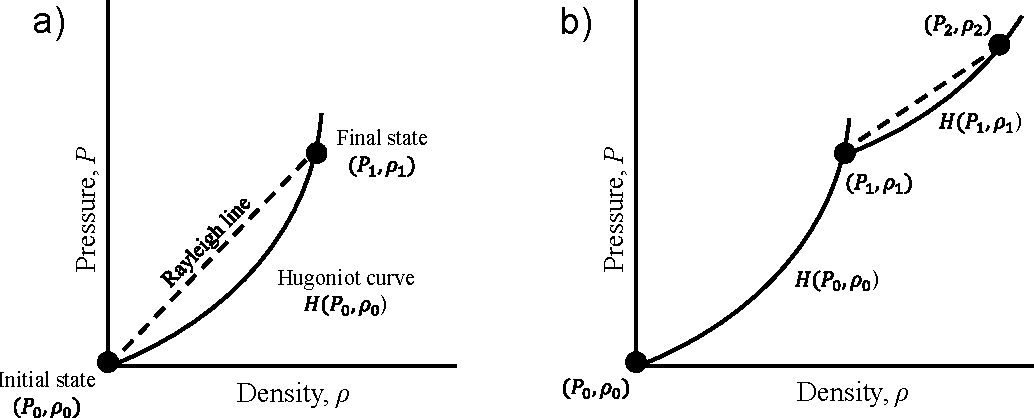
\includegraphics[width=0.8\textwidth]{figures/Theory/SecondaryHugoniot.pdf}% Here is how to import EPS art
\caption{\label{fig:SecondaryHugoniot} a) The principal Hugoniot in $(P, \rho)$ space. A shock compresses material in the intial state along a compression path described by the Rayleigh line to a shock state on the Hugoniot curve. The curve represents the range of possible shock states that could be achieved for a given initial state. b) If a subsequent shock passes through the material, the shock state it will generate lies somewhere on a secondary Hugoniot, which is a unique curve generated for the new initial condition (the shock state achieved by the first shock).}
\end{figure}

The dependence of the Hugoniot on the initial state is significant, as is highlighted in Figure \ref{fig:SecondaryHugoniot}. For the initial state $(P_0, u_0)$, the Hugoniot curve is plotted; this describes the states accessible by a shock from that initial point. Driving a shock with pressure $P_1$ through the target allows the shock state $(P_1, u_1)$ to be achieved. However, following this with a higher shock does not allow a new state on this curve to be accessed, due to the fact that the material ahead of this new shock is no longer $(P_0, u_0)$, is but instead $(P_1, u_1)$. To find the state achieved by this second shock requires a new Hugoniot curve to be plotted, $P_2 = H(P_1, \nu_1, \nu_2)$; this curve will pass through the state $(P_1, u_1)$, and describe the locus of states that the new shock can reach.

The Hugoniot curve describing the states that can be accessed from an initially unshocked material, $P_1 = H(P_0 = 0, \nu_0, \nu_0)$, is particularly significant for two obvious reasons; most materials begin experiments unshocked (and so the first shock state achieved will be on this curve), and the states on this curve are the easiest to measure and access. This curve is known as the `Principal Hugoniot'. This curve can be populated experimentally by measuring the state achieved when shocks of different strengths are passed through initially unshocked material.

It is also worth noting that the Hugoniot curve is not the path that the material takes through $(P, \nu)$ space as it is compressed (rather, it is the possible end states of such a compression). The the compression path is given by a different curve called the `Rayleigh line' \cite{Forbes2012}. The Rayleigh line is described by Equation \ref{eqn: RH2 stationary}, repeated below:
\begin{equation} P_1 - P_0 = \rho_0 U_S u_p.  \end{equation}
Note here that in $(P, u_p)$ space, the Rayleigh line in a straight line with a gradient of $Z = \rho_0 U_S$. If a shock travels through the material with a shock velocity $U_S$, then the final shock state will be the intercept between the Rayleigh line and the Hugoniot. This gradient $Z$ is called the shock impedance , and is significant when considering shocks between different materials. It's also important to note that using Equation \ref{eqn: RH2 stationary} requires all velocities to be in the stationary frame, where the material ahead of the shock is stationary\footnote{In the case shown in Figure \ref{fig:SecondaryHugoniot} (b) where this material ahead of the shock has been preshocked, the `stationary frame' is now moving so that the material ahead of the shock appears stationary. If the material has been preshocked to a pressure $P_a$ and velocity $u_a$, and the new shock moving at $U_S$ drives the material to a pressure $P_b$ and velocity $v_b$, then the Rayleigh line would be given by $P_b - P_a = \rho_0 (U_S - u_a) (u_b - u_a).$ }

\subsection{Material interfaces and impedance matching \label{IMTheory}}

The previous sections have considered shocks moving through a single material - material interfaces will now be considered. This section follows the descriptions given in \cite{Forbes2012} and \cite{Davison2008}. Imagine a shock $S_1$ travelling through material A, which then reaches an interface with material B. Some fraction of the shock energy will be transmitted across the interface into material B, while some will be reflected into material A. The pressure behind the reflected shock $P_R$ is given \cite{Colvin2013} by 
\begin{equation} \frac{P_R}{P_1} = \frac{Z_2 - Z_1}{Z_2 + Z_1}.  \end{equation}
Three illustrative cases are useful to consider. If the impedances of the two materials are very similar $Z_2 \approx Z_1$, the reflected shock pressure will be effectively zero and almost all the shock energy propagates into the new material. If there is a high impedance mismatch between the materials, then a large fraction of the shock energy is reflected. If the new material is higher impedance $Z_2 > Z_1$, then the reflected pressure is positive and a shock is reflected. If the new material is instead low impedance $Z_2 < Z_1$ then the rarefaction/relaxation wave is instead reflected.

The state achieved either side of the interface after the shock crosses it can be found through an impedance matching calculation. This relies on a key principal. After the shock has crossed the interface, the material on either side is in the state achieved by the transmitted/reflected waves $S_2$ and $S_3$. For the two materials to remain in contact, it is required that the pressure $P$ and particle velocity $u_p$ of the material either side of the boundary must be equal - if this were not the case, the boundary would not be in equilibrium, or the two layers would separate. This enables impedance matching calculations, where the state in each material following the shock crossing the interface can be determined.

\begin{figure}
\centering     %%% not \center
\subfigure{a)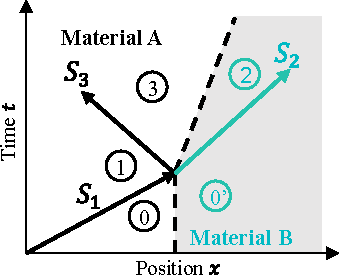
\includegraphics[width=.45\textwidth]{figures/Theory/ShockDiagram.pdf}}
\subfigure{b)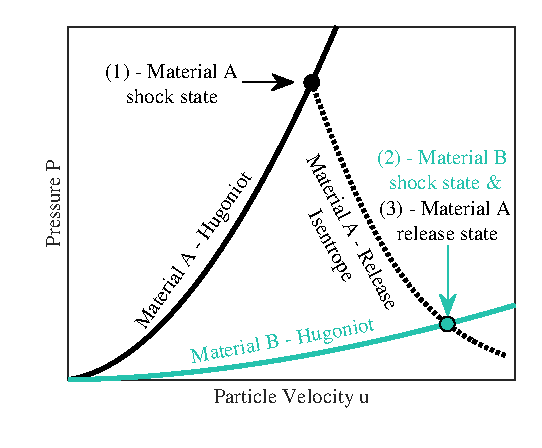
\includegraphics[width=.45\textwidth]{figures/Theory/MatlabIM1.eps}}
\caption{ \label{fig:ShockDiagramAndIMTheory1} a) x-t diagram showing a shock transiting across the interface from a high impedance material into a low one. The dashed line shows the material interface, while the arrows show the shocks. The shock/rarefaction waves are refered to as $S_n$, while the shock states are refered to by the numbers. b) $(P,u)$ plot showing the impedance matching graphically. $S_1$ shocks material in state (0) to a state (1) on the Hugoniot for quartz A. Rarefaction wave $S_3$ causes A to relax from (1) to a state (3) on the release isentrope for A. Shock $S_2$ shocks B from state (0') to state (2) on the foam Hugoniot. The impedance matching criteria means that (2) and (3) are equivalent in $(P,u)$ space, and thus this state is the intercept of these two curves.}
\end{figure}

This is shown graphically for the case where the second material is lower impedance in Figure \ref{fig:ShockDiagramAndIMTheory1}. Two materials, A and B, are in contact with an interface between them. They are both initially unshocked, in states described as (0) and (0') respectively. The pressure and particle velocity of state (0) can be described as $(P_0, u_0)$ - as both (0) and (0') are unshocked and stationary, both $P$ and $u$ are in fact 0. Note here that the velocity $u_n$ is this section is just used to refer to the velocity of the state labelled $n$, rather than suggesting that a particular reference frame is being used - in fact, it is simplest to do the maths in the stationary frame.

An initial shock $S_1$ travels through material A shocking it to the state (1) with $(P_1, u_1)$, which must by definition lie on the principal Hugoniot for material A. $S_1$ reaches the interface between the two materials, and this generates a rarefaction wave $S_3$ which travels back into material A, and a shock wave $S_2$ which propagates through material B. As material B is unshocked, the new state $(P_2, u_2)$ lies on the principal Hugoniot for material B. Rarefaction wave $S_3$ travels through the pre-shocked state $(P_1, u_1)$, and causes it to relax to a new state $(P_3, u_3)$. This relaxation occurs along another curve known as the release isentrope, which describes the locus of states that the material could relax to given it's shocked initial state of $(P_1, u_1)$. 

It is clear from Figure \ref{fig:ShockDiagramAndIMTheory1} (a) that after this shock crossing occurs, the interface is now the contact between the shocked material B in state (2) and lies on the B Hugoniot, and the relaxed material A in state (1) which lies on the A release isentrope. The impedance matching criteria requires that both pressure and particle velocity must be constant across the interface, and as such $P_3 = P_2$ and $u_3 = u_2$. This condition is satisfied at the intercept of these two curves in $(P, u)$ space, as shown in Figure \ref{fig:ShockDiagramAndIMTheory1} (b). Therefore, the intercept of these two curves\footnote{There are two things to note here. 1) There is only one state which satisfies this condition. However, if the shock $S_1$ strength is changed, the state $(P_1, u_1)$ is changed, and thus the release isentrope (which depends on this initial state) also changes - meaning that the impedance matching criteria where the Hugoniot B and release isentrope are satisfied now also occurs at a different point. 2) While the $(P,u)$ state of the two materials is equivalent, the Rankine-Hugoniot equations used to calculate the other variables reference the initial state of the material being considered - meaning that the other shock variables for these materials will not be equal.}. defines both states (2) and (3). 

The general principle is the same if B has a higher impedance than A, but with a few changes. Here, the wave $S_2$ is now a shock wave rather than a rarefaction wave. This means that the state (3) is no longer a relaxed state on the release isentrope, but a new shock state which lies somewhere on a secondary Hugoniot of A (i.e. a Hugoniot generated for the initial conditions of state (1)). This also results in a pressure $P_3 = P_2$ which is greater than $P_1$. However, the impedance matching condition $P_3 = P_2$ and $u_3 = u_2$ still applies, and thus in this case the states (2) and (3) are instead the intercept between the principle Hugoniot of material B with this new secondary Hugoniot of material A (replacing the release isentrope).

\subsection{Measuring shock states experimentally \label{IMTheoryMeasurements}}

%It was shown earlier in this section that the Rankine-Hugoniot relations allow all the shock variables associated with a shock state to be calculated, if at least two of the variables (and the state of the unshocked material) are already known. Experiments to measure shock states therefore require the measurement of any two of these variables. `Absolute' shock state measurements measure two such variables directly. 

%However, impedance matching provides a way to determine the shock state of a material by only measuring one of these variables directly. This relies on the situation described in the previous subsection. A known reference material, which is already well-characterised, is placed in contact with the material of study. Aluminium or quartz are typical examples. A shock is then driven through the reference material, such that it crosses the interface into the material being studied. As discussed, this will result in a shock/rarefaction (depending on the relative impedance) wave propagating back into the reference, and the pressure and particle velocity in the reshocked/relaxed reference and the shocked material of study will be equal.

%This is performed in such a way that the shock velocity can be measured in both materials. The shock velocity in the reference material during the first shock is measured, and this is used to plot the Rayleigh line $P_1 = \rho_0 D u$ in the reference. The intercept of the Rayleigh line and the Hugoniot defines the shock state that the reference material reaches after the first shot. When the reflected shock/rarefaction wave propagates back through the reference, this material will be shocked/relaxed according to an as yet undetermined point somewhere on the known reference Hugoniot/release isentrope. 

%Following the theory in the previous section, it is clear the 

It was shown earlier in this section that the Rankine-Hugoniot relations allow all the shock variables associated with a shock state to be calculated, if at least two of the variables (and the state of the unshocked material) are already known. 'Absolute' shock experiments therefore aim to measure two such variables directly. However, impedance matching experiments make use of the impedance matching criteria to enable the shock state in a material to be determined by measuring only one variable (typically the shock velocity) in two materials; the material of study, and a reference material. This is often simpler experimentally.

\begin{figure}
\centering
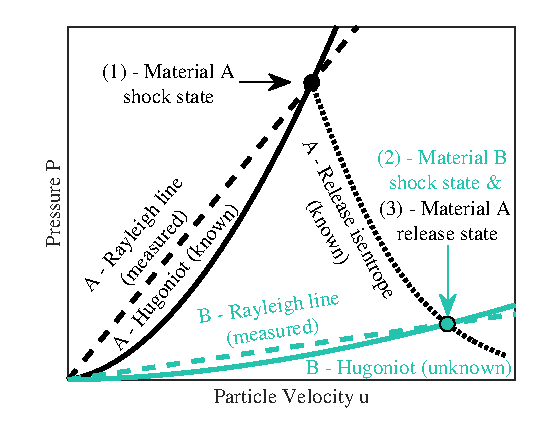
\includegraphics[width=0.6\textwidth]{figures/Theory/MatlabIM2.eps}% Here is how to import EPS art
\caption{\label{fig:IMTheory2} A $(P,u)$ plot as in Figure \ref{fig:ShockDiagramAndIMTheory1}, showing how impedance matching is used experimentally. Material A is a reference, where the Hugoniot and release isentrope are known. Measuring the shock velocity of $S_1$ in A allows the Rayleigh line to be plotted - the intercept of this with the known Hugoniot for A allows state (1) to be determined. Measuring the shock velocity of $S_2$ in B also allows a Rayleigh line to be plotted for this shock. The intercept of this line with the known release isentrope A allows the state (2), a shock state of B which lies on the unknown Hugoniot of B, to be calculated.}
\end{figure}

Consider the situation described in the previous section, but with material A now being a known reference (which means that the relevant curves, such as the Hugoniots and the release isentrope, are already known) and material B is the material of study. Imagine that an experiment is conducted so that the shock velocity of $S_1$ in material A and of  $S_2$ in material B are measured.

Measuring the shock velocity $U_{S_1}$ allows the Rayleigh line for this shock to be plotted. As discussed in Section \ref{The Hugoniot theory}, the achieved shock state in material A will be the intercept of the Rayleigh line and the material Hugoniot. As A is a reference material where the Hugoniot is measured, this intercept can therefore be identified, and the shock state (1) determined. This is shown in Figure \ref{fig:IMTheory2}. This shock state (1) can then be used to calculate the release isentrope\footnote{This example is given again for where B is lower impedance than A. If B is higher impedance, replace all mentions of the isentrope with the secondary Hugoniot, and any mention of `relaxed' material A to `reshocked' material A.} for material A. Again, as A is a reference, this isentrope is already known.

Measuring the shock velocity $U_{S_2}$ enables the Rayleigh line for the shock in material B $S_2$ to be plotted, and the intercept with the Hugoniot for material B would define the shock state for that material. As material B is the material for which the shock behaviour is being investigated, this Hugoniot is not known. Howver, the impedance matching criteria means that this is the same $(P, u)$ state achieved in the relaxed (or reshocked) material A, and thus also lies on the release isentrope for this material. The shock state (2) of material B can therefore be identified from the intercept of the release isentrope for A and the Rayleigh line for B. This shock state is thus determined through only measurements of the two shock velocities, and knowledge of the reference material.

\section{Theory of compression for EOS?}